\chapter{Mantle: Subtree Load Balancing}
\label{mantle}

% Multi-MDS problem: synchronizing access and coalescing knowledge 
The most common technique for improving the performance of metadata services is
to balance the load across a cluster of metadata server (MDS)
nodes~\cite{patil:fast2011-giga+, weil:osdi2006-ceph, weil:sc2004-dyn-metadata,
sinnamohideen:atc2010-ursa, xing:sc2009-skyfs}.  Distributed MDS services focus
on parallelizing work and synchronizing access to the metadata. A popular
approach is to encourage independent growth and reduce communication, using
techniques like lazy client and MDS synchronization~\cite{patil:fast2011-giga+,
ren:sc2014-indexfs, zheng:pdsw2014-batchfs, hildebrand:msst2005-pnfs,
zhu:pds2008-hba}, inode path/permission caching~\cite{brandt:mss2003-lh,
li:msst2006-dynamic, xing:sc2009-skyfs}, locality-aware/inter-object
transactions~\cite{sinnamohideen:atc2010-ursa,zhu:pds2008-hba,ren:atc2013-tablefs,
ren:sc2014-indexfs} and efficient lookup tables~\cite{brandt:mss2003-lh,
zhu:pds2008-hba}. Despite having mechanisms for migrating metadata, like
locking~\cite{sinnamohideen:atc2010-ursa,schmuck:fast2002-gpfs}, zero copying
and two-phase commits~\cite{sinnamohideen:atc2010-ursa}, and directory
partitioning~\cite{xing:sc2009-skyfs, patil:fast2011-giga+, ren:sc2014-indexfs,
weil:osdi2006-ceph}, these systems fail to exploit locality.

\begin{figure}[tb]
	\centering	
	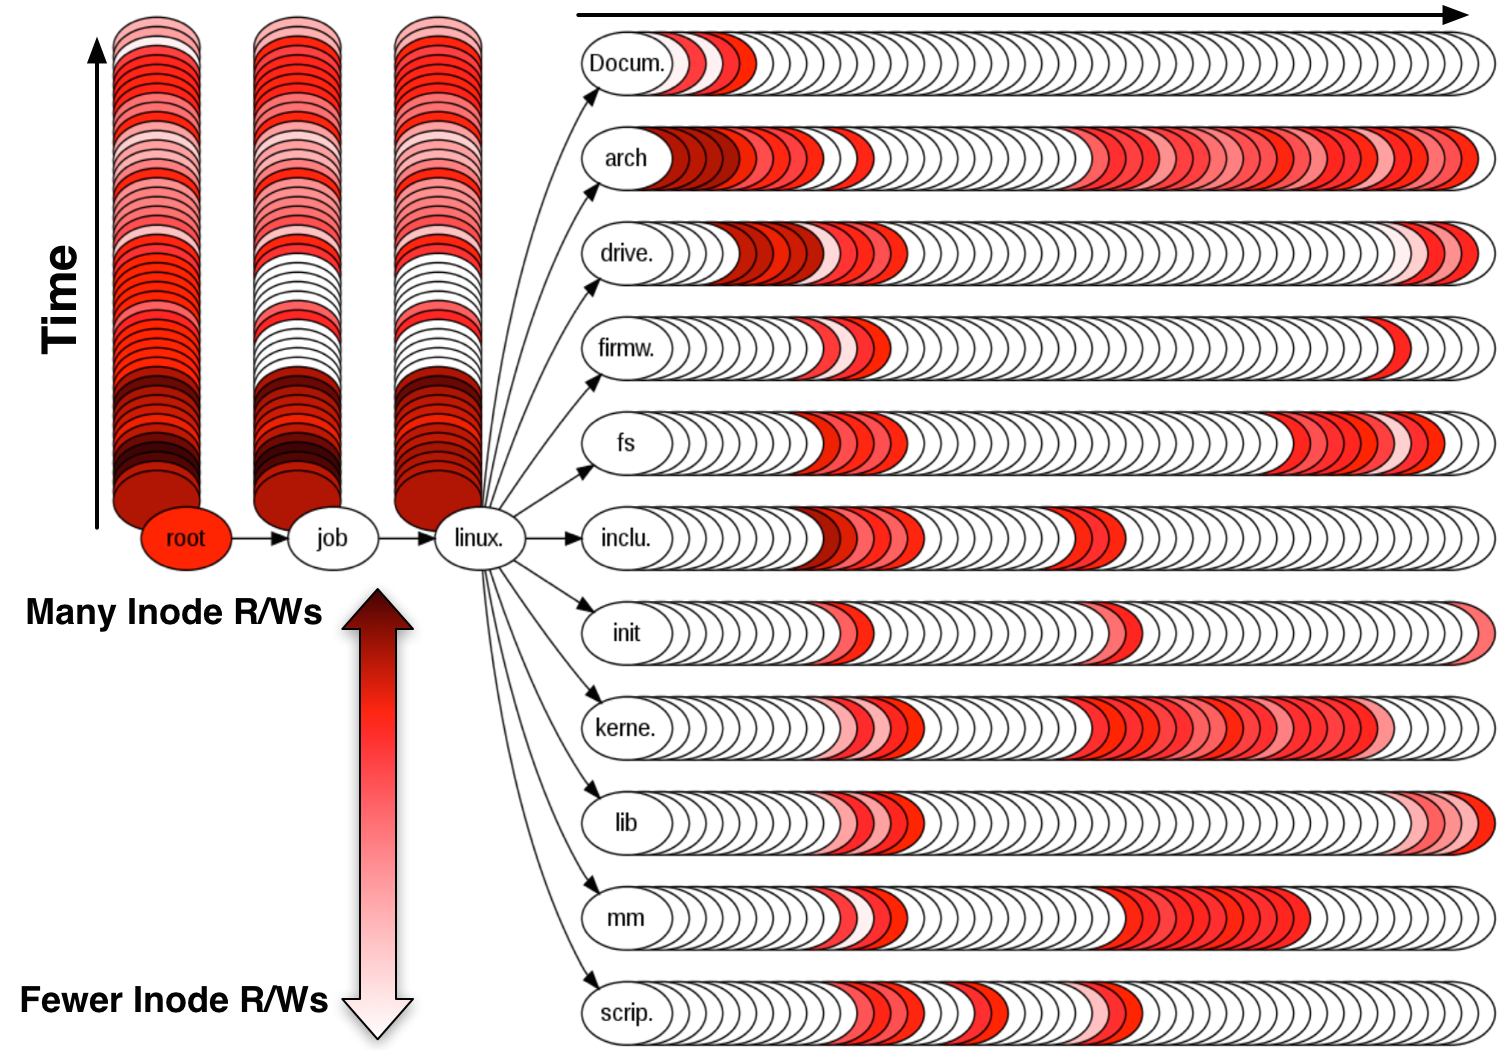
\includegraphics[width=0.5\textwidth]{./chapters/mantle/figures/workload-tar.png}
	\caption{Metadata hotspots, represented by different shades of red, have spatial and temporal locality when compiling the Linux source code. The hotspots are calculated using the number of inode reads/writes and smoothed with an exponential decay. \label{figure:workload-tar}}
\end{figure}

% ... and what we do
We envision a general purpose metadata balancer that responds to many types of
parallel applications. To get to that balancer, we need to understand the
trade-offs of resource migration and the processing capacity of the MDS nodes.
We present Mantle\footnote{The mantle is the structure behind an octopus's head
that protects its organs.}, a system built on CephFS that exposes these factors
by separating migration policies from the mechanisms. Mantle accepts injectable
metadata migration code and helps us make the following contributions:

\begin{itemize}

    \item a comparison of balancing for locality and balancing for distribution

    \item a general framework for succinctly expressing different load
    balancing techniques 

    \item an MDS service that supports simple balancing scripts using this
    framework

\end{itemize}

Using Mantle, we can dynamically select different techniques for distributing
metadata. We explore the infrastructures for a better understanding of how to
balance diverse metadata workloads and ask the question ``is it better to
spread load aggressively or to first understand the capacity of MDS nodes
before splitting load at the right time under the right conditions?''. We show
how the second option can lead to better performance but at the cost of
increased complexity. We find that the cost of migration can sometimes outweigh
the benefits of parallelism (up to 40\% performance degradation) and that
searching for balance too aggressively increases the standard deviation in
runtime.
